\documentclass[reprint]{revtex4-1}
\usepackage{amsmath,amssymb}
\usepackage{graphicx}
\usepackage{cleveref}
\usepackage{standalone}
\usepackage{siunitx}

\begin{document}
\title{Ignition and Extinction Characteristics of a Capacitively Coupled Plasma}
\author{Daniel Underwood}
\date{\today}

\begin{abstract}

\end{abstract}
\maketitle

\section{Introduction}
Plasmas are quasineutral substances consisting of ionized atoms and the electrons removed from those atoms. Due to the quasineutral nature of plasmas, electromagnetic fields outside of the plasma are negligible while the internal fields are extremely complex. While rather rare on Earth, plasmas are ubiquitous throughout the rest of the universe \cite{F.F.Chen1989}.

In our experiment, we continue the previous work of Mann and Morton \cite{Mann2015} by generating an RF signal between two electrodes, which creates a capacitively coupled plasma (CCP) between the plates with a Debye sheath at the plates, as shown in \cref{fig:plasma-sheath}.

In this paper, we will examine the equipment and errors in our experimental setup, present the results we have collected, discuss those results, and conclude with final thoughts and direction for future work.

\begin{figure}
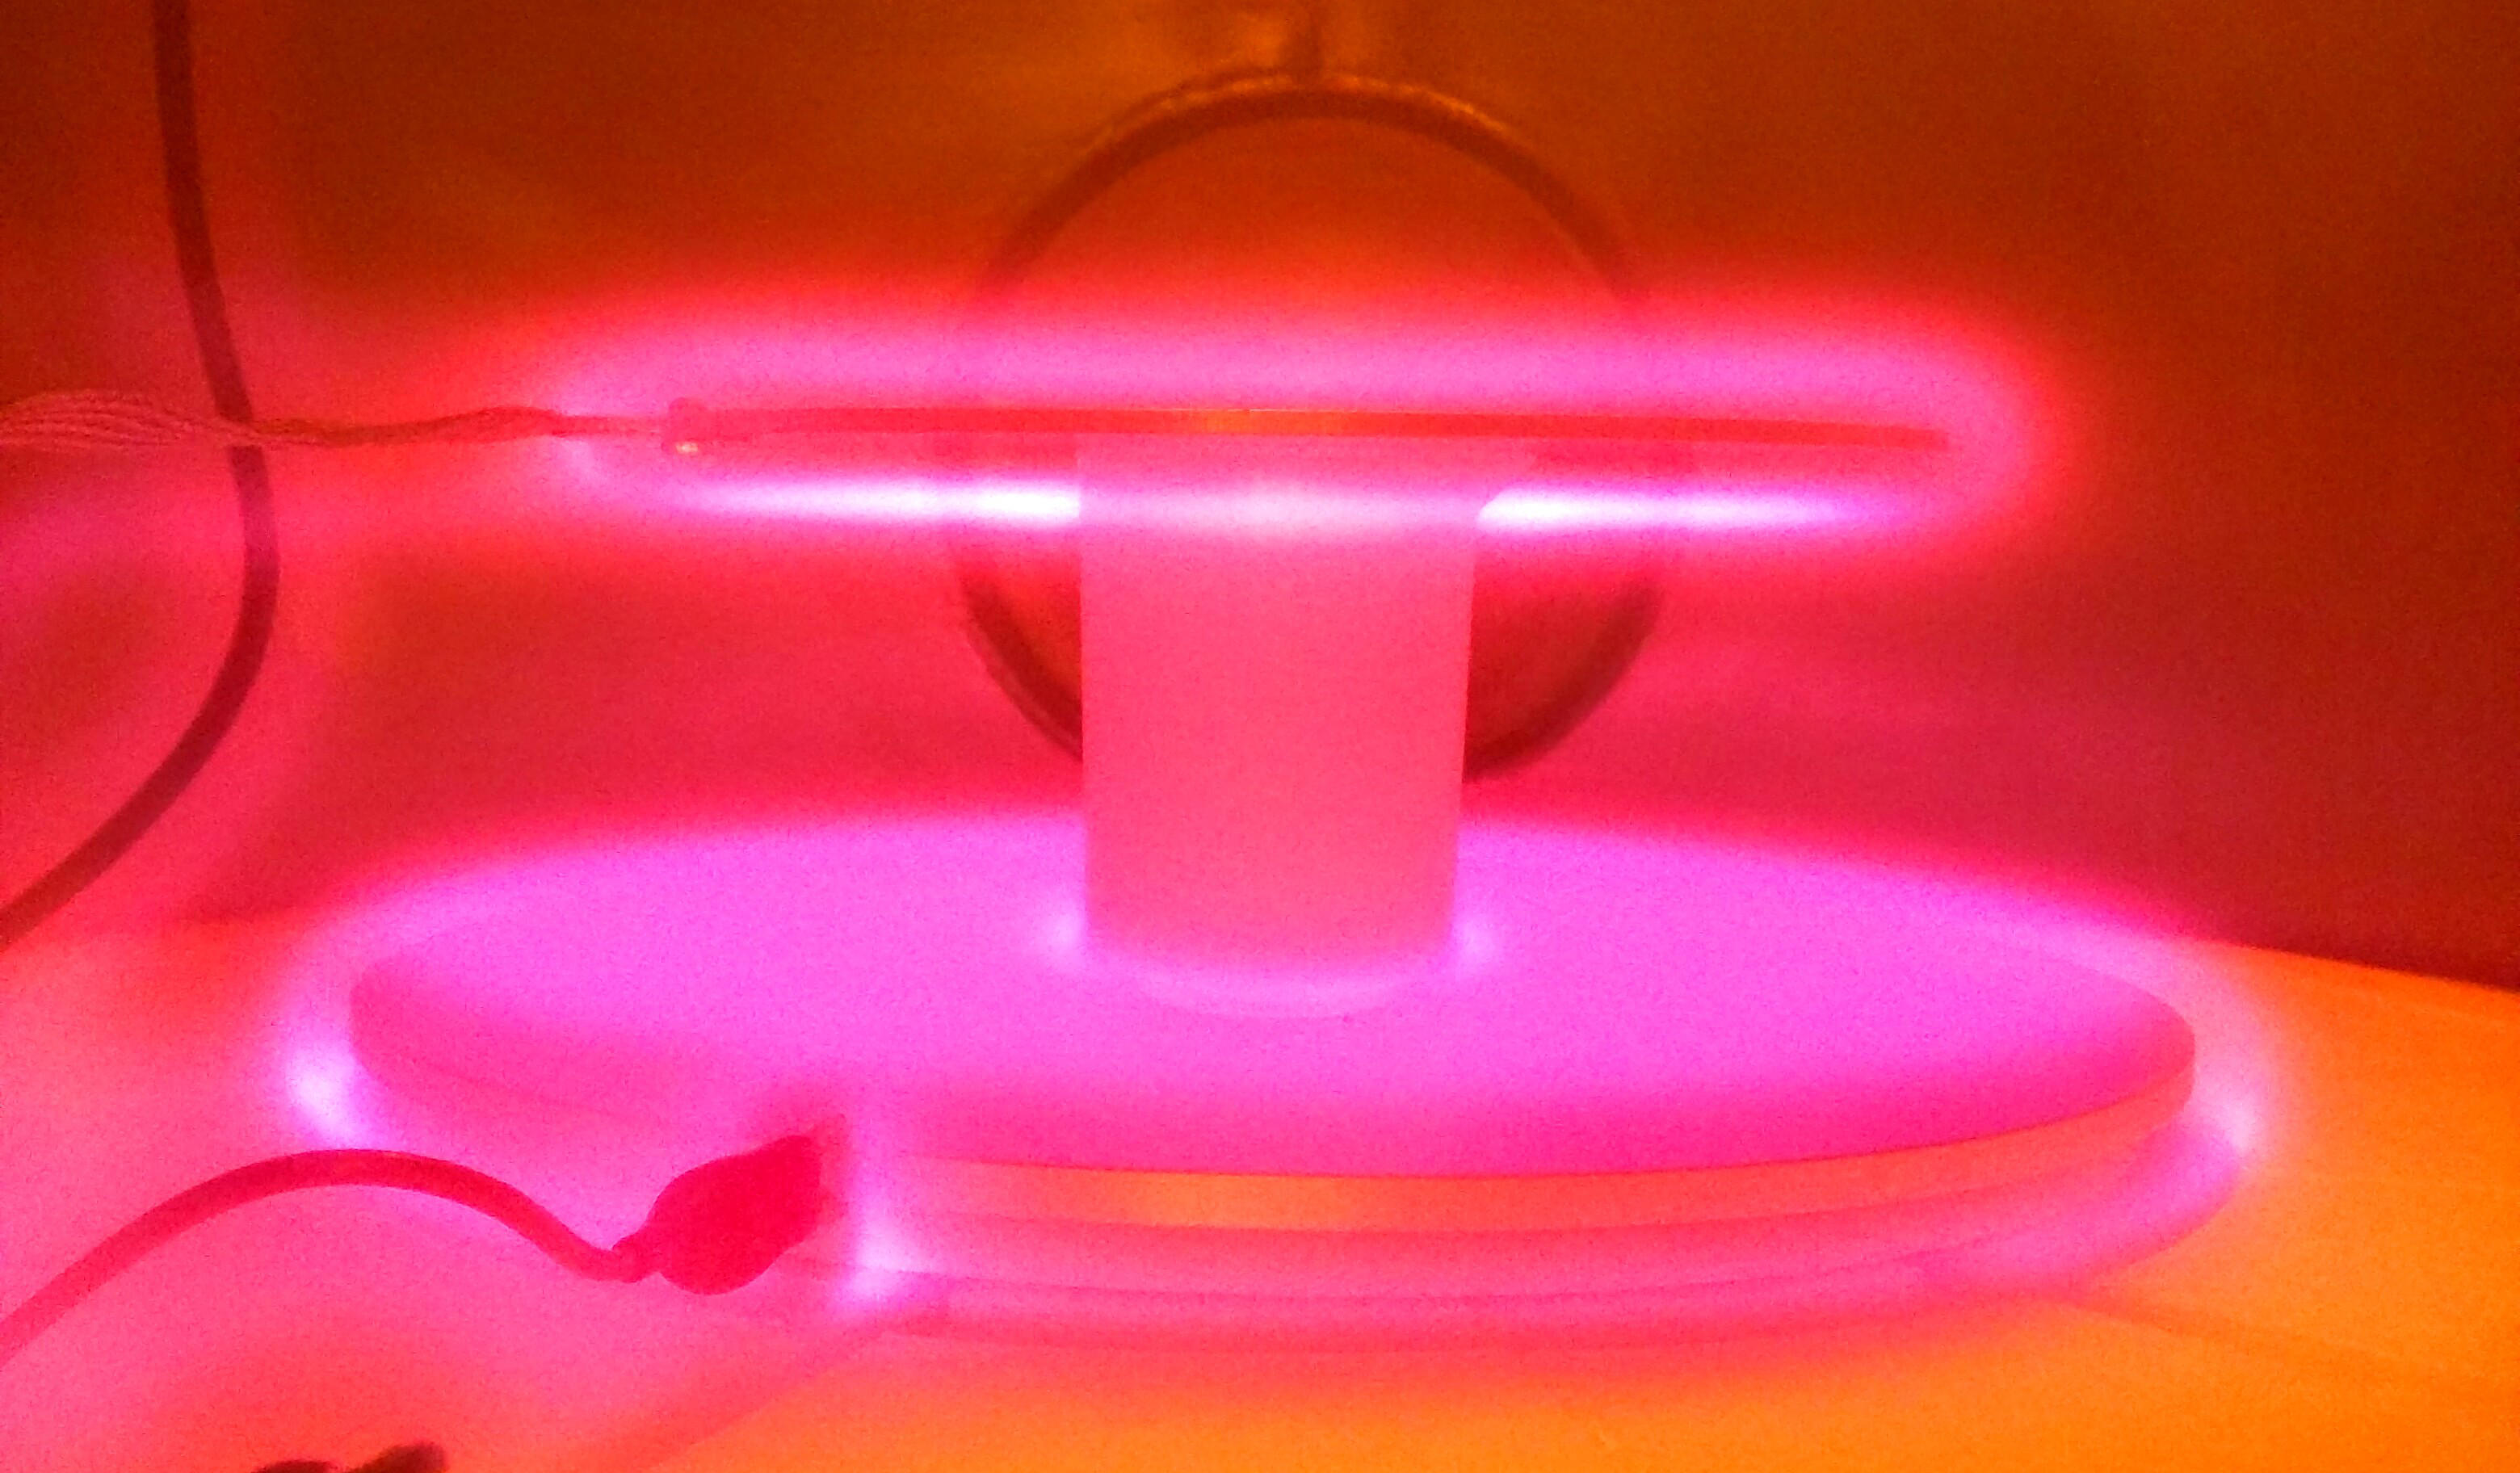
\includegraphics[width=\columnwidth]{../resources/plasma-sheath.png}
\caption{(Color Online) Capacitor plates and Debye sheath}
\label{fig:plasma-sheath}
\end{figure}

\section{Methods}

The plasma was generated within a vacuum chamber at a pressure on the order of $10^{-1}\:\rm{Torr}$. Plasma was generated by applying an RF signal between two plates separated by a distance of $8.6 \pm 0.1\:\rm{cm}$. The RF signal was generated by a Dressler Cesar RF Power Generator $13.56\:\rm{MHz}$ $300\:\rm{W}$ attached to an ENI Automatic Matching Network to account for reflected signals. This setup creates a capacitively coupled plasma (CCP) \cite{physics-radio-frequency}, which creates a plasma between the capacitor plates with Debye sheaths at the plates, as shown in \cref{fig:plasma-sheath}.  A Tektronic TDS 1002 oscilloscope was used to measure the voltage between the two plates with a 100X probe; data was recorded manually and statistical uncertainties were taken to be the maximum change from the mean value over a two second interval. It should be noted that this is likely an overestimation of error as it is the range rather than the standard deviation of the data; this could result in errors in data analysis and overfitting of the data.

\section{Results}

\section{Discussion}

\section{Conclusion}

In the context of an educational laboratory, our experiment may be improved by continually taking measurements of the power and voltage in order to obtain the information necessary to have an IV curve for the plasma and subsequently extract IV characteristics from the plasma. In addition to our setup of a capacitively coupled plasma,  the equipment may be used to generate an inductively coupled plasma by replacing the electrode plates with a solenoid and modifying the vacuum system to pump along the axis of the solenoid, as described in \cite{physics-radio-frequency,Jiayin2010}.

\bibliography{plasma-iv-characteristics}

\end{document}